\documentclass[11pt]{article}    % тип дока
\usepackage[utf8]{inputenc}   % используемые языки
\usepackage[T2A]{fontenc}   % используемые языки
\usepackage[english, russian]{babel}   % используемые языки
\usepackage[14pt]{extsizes}   % размер шрифта 14pt
\usepackage[a4paper, left=3cm, right=1cm, top=2cm , bottom=2cm]{geometry}
\usepackage{indentfirst}   % красная строка даже в первом абзаце
\usepackage{graphicx}
\usepackage{xcolor} % пакет для работы с цветами
\usepackage{amssymb}
\usepackage{amsmath}
\usepackage{amsfonts}
\usepackage{hyperref}
%\usepackage{stmaryrd}
\linespread{1.5}   % межстрочный интервал 1.5


\begin{document}

\begin{titlepage}
    
\includegraphics[scale = 0.43]{alf4.JPG}
    \\

НАПРАВЛЕНИЕ 03.03.01 Прикладные математика и физика
\par ПРОФИЛЬ Теоретическая Физика\\

\begin{center}
\begin{bf}
     ЗАДАНИЕ\\ 
     о прохождении производственной практики (НИР)
\end{bf}
  


студента Кононова Александра Михайловича \\

Курс 3 Группа 301.3
\end{center}

Форма обучения: очная \\
Сроки прохождения практики с 01.07.2025 по 14.08.2025 \\
Форма представления на кафедру выполненного задания: 
отчет в письменной форме\\
Дата выдачи задания: 01.07.2025\\
Задание для прохождения производственной практики (НИР):
Расчет когерентной суперпозиции испускаемых и резонансно рассеянных фотонов в двухуровневой системе, управляемой импульсным полем. \\
С заданием ознакомлен \\
 
Оценка \\
Руководитель практики Крайнов И.В.\\
(Ф.И.О. полностью, должность, звание, подпись).

\end{titlepage}

\begin{titlepage}


\includegraphics[scale = 0.43]{alf4.JPG}

\

\

\

\

\

\

\begin{center}
    {\bf ОТЧЕТ по производственной практике (НИР)}

    {\bf Весенний семестр 2024/2025 учебного года}

    {\bf Тема: Расчет когерентной суперпозиции испускаемых и резонансно рассеянных фотонов в двухуровневой системе, управляемой импульсным полем.}

\end{center}

    {\bf Студент: Кононов Александр Михайлович}

    {\bf Руководитель практики: Крайнов Игорь Вадимович}

    {\bf Должность, звание:}

    {\bf Оценка:}

\end{titlepage}

\tableofcontents
\newpage

\section{Введение}
\subsection{Актуальность}

Мы представляем результаты о наблюдении группы фотонов в состояниях,
содержащих $\sim$ 3 фотона, представляющих собой когерентную суперпозицию
излученных и резонансно рассеянных лазерных фотонов. Данное явление
возникает при возбуждении двухуровневой системы — заряженной квантовой
точки в микроровезонаторе — импульсами с площадью, кратной 2$\pi$.
Возникновение явления обусловлено тем, что возбуждающий лазерный импульс
содержит несколько десятков фотонов, чье амплитудное квантовое
распределение формирует такую суперпозицию, а поляризация рассеянных
фотонов изменяется в результате взаимодействия с заряженной резонансной
системой. Подобный пучок фотонов является состоянием высшего порядка в
Фоковском пространстве и перспективен для применения в квантовых
технологиях.
%{\color{blue} Так окрашивается текст}
\subsection{Цель и задачи практики}

{\bfЦель:} 

Получить зависимость $g^{(2)}(0)$ фактора от площади возбуждающего импульса в двух-уровневой системе.
\\

{\bfЗадачи:} 
\begin{itemize}
    \item Найти волновую функции выходного состояния двух-уровневой системы, совпадающей по энергии с частотой импульса
    \item Найти $g^{(2)}(0)$ фактор в двух-уровневой системе, совпадающей по энергии с частотой импульса
    \item Найти волновую функции выходного состояния двух-уровневой системы, НЕ совпадающей по энергии с частотой импульса
    \item Найти $g^{(2)}(0)$ фактор в двух-уровневой системе, НЕ совпадающей по энергии с частотой импульса
\end{itemize}


\newpage

\section{Ход выполнения задания}

\subsection{Нахождение волновой функции выходного состояния двух-уровневой системы, совпадающей по энергии с частотой импульса}
Гамельтониан описывающий двух-уровневою систему имеет вид:
\begin{equation}
    \hat{H} = E_0 \ \hat{a}^{\dag}_{+} \hat{a}_{+} + \omega_0 \ \hat{b}^{\dag}_{-} \hat{b}_{-} +  g \left( \hat{a}^{\dag}_{+} \hat{b}_{-} + \hat{a}_{+} \hat{b}^{\dag}_{-} \right)
\end{equation}
Заметим, что гамельтониан взаимодействует с Фоковским пространством через 2-мерные подпространства с базисом $ \left|  0; N \right>$ и $ \left| 1; N-1 \right>$.
\begin{equation}
    \hat{H} =
\begin{pmatrix}
    \omega_0 N & g\sqrt{N} \\
    g\sqrt{N} & E_0 + \omega_0 (N-1)
\end{pmatrix}
\end{equation}
Найдем собственные числа и вектора, учтя что $E_0$ и $\omega_0$ равны:
\begin{gather}
    \varepsilon^{\pm}_{N} = \omega_0 N \pm g\sqrt{N} \\
    v_{\pm} = \frac{1}{\sqrt{2}} \left( \left|  0; N \right> \pm \left| 1; N-1 \right> \right)
\end{gather}
Двух-уровневая система накачивалась когерентным лазерным излучением с горизонтальной поляризацией.
Волновая функция такой накачки следующая:

\begin{equation}
    \left| \psi_{in} \right> = e^{-\left| \alpha \right|^2 / 2} e^{\alpha \hat{b}^{\dag}_H} \left| 0 \right> = e^{-\left| \alpha \right|^2 / 2} \sum_n \frac{\alpha^n}{\sqrt{n!}}  \left| n_H \right>
\end{equation}
Где $ |\alpha|^2 = N $.
\par Взаимодействие двух-уровневой системы с накачкой описывается оператором эволюции:
\begin{equation}
    \hat{S_0} = \exp\left( -i \tau \hat{H} \right)
\end{equation}
Где $ \tau $ - это время взаимодейтсвия между трионом и ипульсом.
Так как:
\begin{equation}
    \hat{b}^{\dag}_{\pm} = \left( \hat{b}^{\dag}_{H} \pm i \hat{b}^{\dag}_{V} \right) / \sqrt{2}
\end{equation}
то
\begin{gather}
    \left| \psi_{out} \right> = \hat{S_0} \left| \psi_{in} \right> = e^{-\left| \alpha \right|^2 / 2} \ e^{\alpha \hat{b}^{\dag}_{+} / \sqrt{2}} \ \hat{S_0}  \ e^{\alpha \hat{b}^{\dag}_{-}} \ \left| 0 \right>
\end{gather}

Воспользуемся свойством собственных векторов и разложением по базису:

\begin{gather}
    \exp\left( -i \tau \hat{H} \right) \ \left| \psi_{n} \right> = \exp\left( -i \tau E_n \right) \ \left| \psi_{n} \right> \\
    v_{\pm} = \frac{1}{\sqrt{2}} \left( \left|  0; N \right> \pm \left| 1; N-1 \right> \right)
\end{gather}
получим:

\begin{gather} \nonumber
    \left| \psi_{out} \right> = \frac{e^{-\left| \alpha \right|^2 / 2} \ e^{\alpha \hat{b}^{\dag}_{H}}}{2} \sum_n e^{-\alpha \hat{b}^{\dag}_{-} / \sqrt{2}} \left[ \left( \frac{ \left( \frac{\alpha}{\sqrt{2}} \ e^{-i \tau \omega_0 } \ e^{-i \frac{\tau g}{2\sqrt{N}}} \right)^n}{n!}  \ e^{-i \tau g \sqrt{N} / 2} \right. \right. + \\ \nonumber
    +  \left. \frac{ \left( \frac{\alpha}{\sqrt{2}} \ e^{-i \tau \omega_0 } \ e^{i \frac{\tau g}{2\sqrt{N}}} \right)^n }{n!} \ e^{i \tau g \sqrt{N} / 2} \right) \hat{b}^{\dag \ n}_{-} + \\ \nonumber
    + \left( \frac{ \left( \frac{\alpha}{\sqrt{2}} \ e^{-i \tau \omega_0 } \ e^{-i \frac{\tau g}{2\sqrt{N}}} \right)^{n-1}}{\sqrt{n!} \sqrt{\left( n-1 \right)!} }  \ e^{-i \tau g \sqrt{N} / 2}  \right. - \\
    - \left. \left. \frac{ \left( \frac{\alpha}{\sqrt{2}} \ e^{-i \tau \omega_0 } \ e^{i \frac{\tau g}{2\sqrt{N}}} \right)^{n-1}}{\sqrt{n!} \sqrt{\left( n-1 \right)!} }  \ e^{i \tau g \sqrt{N} / 2} \right) \hat{b}^{\dag \ n-1}_{-} \ \hat{a}^{\dag}_{+}\right] \left| 0 \right>
\end{gather}
В этом уравнении мы разложили $\sqrt{n}$ до линейного порядка вокруг $N$, для большого среднего значения числа фотонов $\left( N >> 1 \right)$

Так как: $\tau g << 1$, $ |\alpha|^2 = N $ то:

\begin{gather} \nonumber
    \left| \psi_{out} \right> = \frac{e^{-\left| \alpha \right|^2 / 2} \ e^{\alpha \hat{b}^{\dag}_{H}}}{2}  \left[ \left( e^{-i \delta \hat{b}^{\dag}_{-} } \ e^{-i \theta / 2} + e^{i \delta \hat{b}^{\dag}_{-} } \ e^{i \theta / 2} \right) \right. + \\
    + \left. \left( e^{-i \delta \hat{b}^{\dag}_{-} } \ e^{-i \theta / 2} - e^{i \delta \hat{b}^{\dag}_{-} } \ e^{i \theta / 2} \right) \hat{a}^{\dag}_{+} \right] \left| 0 \right>
\end{gather}
где: $\theta = \tau g \sqrt{N}$ , $\delta = \frac{\tau g \alpha}{2 \sqrt{2N}}$

Снова разложим до 1 порядка по $ \delta$, а так же учтем, что детектирование испущенных фотонов происходит в вертикальной поляризации

\begin{gather}
    \left| \psi_{out}^V \right> \approx \cos \left( \frac{\theta }{2} \right) \left| 0 \right> + \frac{i \delta - 1}{\sqrt{2}} \sin \left( \frac{\theta}{2} \right) \left| 1 \right> + \frac{i \delta}{2} \cos \left( \frac{\theta}{2} \right) \left| 2 \right>
\end{gather}

\subsection{Расчет $g^{(2)}(0)$ фактора в двух-уровневой системе, совпадающей по энергии с частотой импульса}
%\newpage
Рассчитаем вероятность обнаружить фотон:

\begin{gather}
    P_1 \left( t \right) = \sum_m \left| \left< m \left| \ \hat{a} \ \right| \psi_{out}^V \right> \right|^{2} = \frac{e^{-\left| \alpha \right|^2}}{2} \cdot \sum_m \frac{\alpha^{2m+2}}{\left( m+1 \right)!} \left( 1 - \cos \left( 2gt \sqrt{m+1} \right) \right)
\end{gather}

\par
\begin{center}
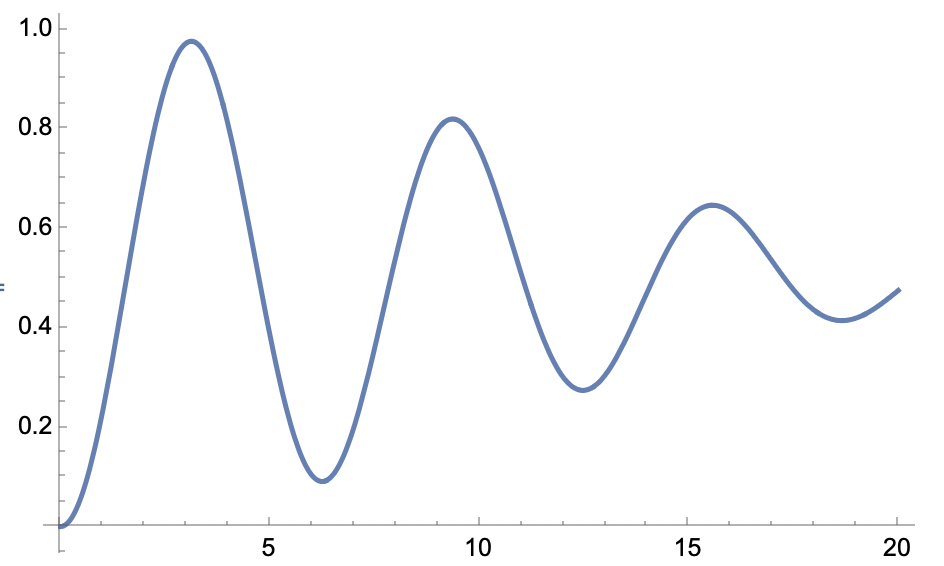
\includegraphics[scale = 0.75]{plot1.png}
\par
    \underline{Рисунок 1}: $P_1 \left( t \right)$ - вероятность обнаружить фотон
\end{center}
\par

$g^{(2)}(0)$ фактор показывает вероятность обнаружить 2 когерентных фотона одновременно. Он считается следующим образом:

\begin{gather}
    g^{(2)}(0) = \frac{ \left< \psi_{out}^V \left| \ \hat{n}^2 - \hat{n} \ \right| \psi_{out}^V \right>}{\left< \psi_{out}^V \left| \ \hat{n}^2 \ \right| \psi_{out}^V \right> ^2 } = \frac{2\left| \delta \right|^2 \cos^2 \left( \frac{\theta}{2} \right) }{\sin^2 \left( \frac{\theta}{2}\right) + \left| \delta \right|^2}
\end{gather}


\par
\begin{center}
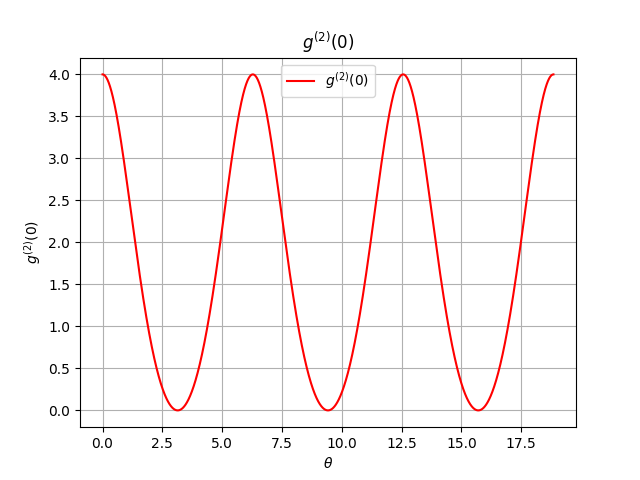
\includegraphics[scale = 1]{plot2.png}
\par
    \underline{Рисунок 2}: $g^{(2)}(0)$
\end{center}
\par Видно, что $g^{(2)}(0)$ становится равным 0 при нечетных площадях импульса $(\pi, 3\pi, \dots)$ и имеет максимум при нечетных площадях импульса $(2\pi, 4\pi, \dots)$

\subsection{Нахождение волновой функции выходного состояния двух-уровневой системы, НЕ совпадающей по энергии с частотой импульса}
В этой задачи условия похожи, однако теперь $E_0 \neq \omega_0 $.
\par Гамельтониан:

\begin{gather}
\hat{H} =
\begin{pmatrix}
    \omega_0 N & g\sqrt{N} \\
    g\sqrt{N} & E_0 + \omega_0 (N-1)
\end{pmatrix}
\end{gather}

Собственные числа и вектора:

\begin{gather}
    \varepsilon^{\pm}_{N} = \omega_0 N + \frac{1}{2} \left( E_0 - \omega_0 \right) \pm \sqrt{\left( E_0 - \omega_0 \right)^2 + 4 g^2 N} \\ \nonumber
    v_{\pm} = \frac{1}{\sqrt{1+\left( \frac{\frac{1}{2} \left( E_0 - \omega_0 \right) \pm \sqrt{\left( E_0 - \omega_0 \right)^2 + 4 g^2 N}}{g\sqrt{n}} \right)^2 }} \cdot \\
    \cdot \left( \left|  0; N \right> + \left( \frac{1}{2} \left( E_0 - \omega_0 \right) \pm \sqrt{\left( E_0 - \omega_0 \right)^2 + 4 g^2 N} \right) \left| 1; N-1 \right> \right)
\end{gather}

Проделав все те же шаги, получим волновую функцию после взаимодействия накачки и двух-уровневой системы:

\begin{gather} \nonumber
    \left| \psi_{out}^V \right> = \frac{e^{-\left| \alpha \right|^2 / 2} \ e^{\alpha \hat{b}^{\dag}_{H}}}{2\sqrt{1+\delta_N^2}}  \left[ e^{-i \theta / 2 } \ e^{-i \gamma \hat{b}^{\dag}_{-} } \left( \sqrt{1+\delta_{N}^2} - \delta_N \right) \right. + \\ \nonumber
    + e^{i \theta / 2 } \ e^{i \gamma \hat{b}^{\dag}_{-} } \left( \sqrt{1+\delta_N^2} + \delta_N \right) + \\
    + \left. \left( e^{-i \theta / 2 } \ e^{-i \gamma \hat{b}^{\dag}_{-} } - e^{i \theta / 2 } \ e^{i \gamma \hat{b}^{\dag}_{-} } \right) \hat{a}^{\dag}_{+} \right] \left| 0 \right>
\end{gather}

Где $\delta_n = \frac{E_0 - \omega_0}{2g\sqrt{n}} $, $\theta = \tau g \sqrt{N}\sqrt{1+\delta_N^2} $, $\gamma = \frac{\tau g \alpha }{2\sqrt{2N}} $.

Разложим до линейного порядка по $\gamma$, а так же учтем смену поляризации

\begin{gather} \nonumber
    \left| \psi_{out}^V \right> \approx \frac{e^{-\left| \alpha \right|^2 / 2}}{\sqrt{1+\delta_N^2}} \left[ \left( \sqrt{1+\delta_N^2} \cdot \cos\frac{\theta}{2} + i \delta_N \sin\frac{\theta}{2}  \right) \left| 0 \right> + \right. \\
    \left. + \left( \frac{i \gamma \sqrt{1+\delta_N^2} - 1 }{\sqrt{2}} \sin\frac{\theta}{2} + \frac{\delta_N \gamma}{\sqrt{2}} \cos\frac{\theta}{2} \right) \left| 1 \right> +  \frac{i\gamma}{2} \cos\frac{\theta}{2} \left| 2 \right> \right]
\end{gather}

\subsection{Расчет $g^{(2)}(0)$ фактора в двух-уровневой системе, НЕ совпадающей по энергии с частотой импульса}

\begin{gather}
    g^{(2)}(0) = \frac{ \left< \psi_{out}^V \left| \ \hat{n}^2 - \hat{n} \ \right| \psi_{out}^V \right>}{\left< \psi_{out}^V \left| \ \hat{n}^2 \ \right| \psi_{out}^V \right> ^2 } = \frac{2 \left( 1+\delta_N^2 \right) \gamma^2 \cos^2 \frac{\theta}{2} }{\left( \gamma^2 \left( 1 + \delta_N^2 \right) + \sin^2 \frac{\theta}{2} - \delta_N \gamma \sin \theta \right)^2}
\end{gather}

Видим, что при $ \delta_N  \rightarrow \infty \Rightarrow g^{(2)}(0) \rightarrow 0 $. Это хороший и логичный результат, означающий что при большой разности энергий взаимодействие не происходит.

Построим зависимость $g^{(2)}(0)$ от $\delta_N$ при разных площадях импульса $\theta$:
\par
\begin{center}
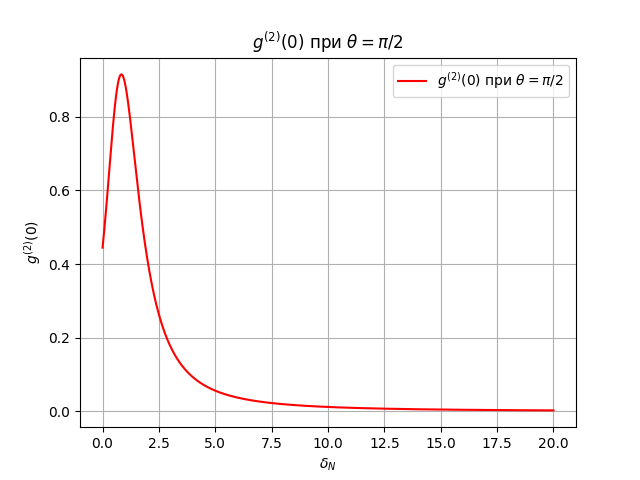
\includegraphics[scale = 0.8]{plot3.png}
\par
    \underline{Рисунок 3}: $g^{(2)}(0)$ при $\theta = \pi/2$
\end{center}
\par
\begin{center}
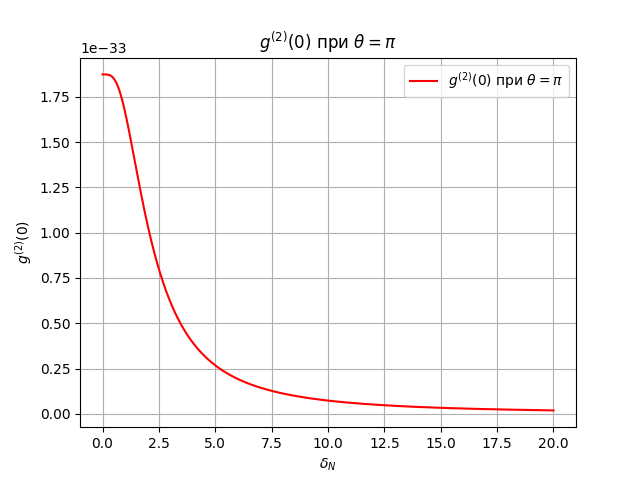
\includegraphics[scale = 0.8]{plot4.png}
\par
    \underline{Рисунок 4}: $g^{(2)}(0)$ при $\theta = \pi$
\end{center}
\par
\begin{center}
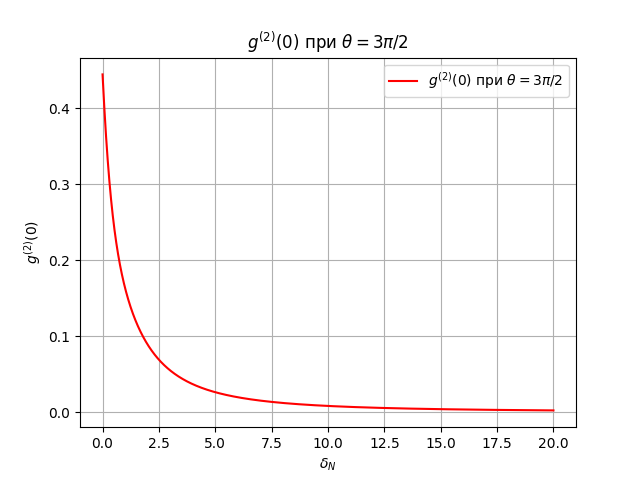
\includegraphics[scale = 0.8]{plot5.png}
\par
    \underline{Рисунок 5}: $g^{(2)}(0)$ при $\theta = 3\pi/2$
\end{center}
\par
\begin{center}
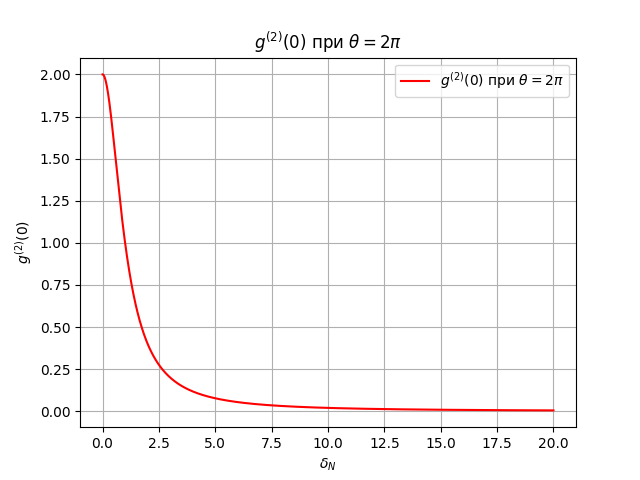
\includegraphics[scale = 0.8]{plot6.png}
\par
    \underline{Рисунок 6}: $g^{(2)}(0)$ при $\theta = 2\pi$
\end{center}
\par

\section{Заключение}
В данной работе мы исследовали генерацию многофотонных состояний в системе — заряженной квантовой точке,
расположенной в микрорезонаторе, возбуждаемой четными $\pi$‑импульсами.
Экспериментально полученные данные демонстрируют,
что при такой форме возбуждения наблюдается скучивание двухфотонного состояния,
что свидетельствует о когерентной суперпозиции излучённых и резонансно рассеянных фотонов.

Формирование таких состояний с гибко настраиваемой статистикой открывает широкие возможности для развития квантовых технологий,
включая схемы квантовых вычислений и протоколы квантового распределения ключей.
Данный подход предполагает эффективное управление статистикой фотонных состояний через форму и мощность возбуждающих импульсов и свойства резонансной системы.

\section{Список литературы}

   \begin{enumerate}
       \item Krainov I.V., 'Coherent superposition of emitted and resonantly scattered photons from a two-level system driven by an even-$\pi$ pulse', Mesoscale and Nanoscale Physics (2025)
       \item Marlian O. Scully and M. Suhail Zubairy, 'Quantum optics' (1996)
       \item Bonch-Bruevich V.L., 'Physics of Semiconductors' (1965)
       \item Anselm A.I., Introduction to Semiconductor Theory (1963)
   \end{enumerate}

\end{document}
